\section{Introdução ao controle de processos industriais}

\begin{frame}{Introdução}
	\begin{block}{O que é a teoria de controle?}
		\begin{itemize}
			\item Trata-se do estudo de \textbf{como} levar um processo a um ponto de equilíbrio, ou seja, à \textbf{estabilidade}.
			\item Seja no piloto automático de um avião, ou na indústria, a \textbf{teoria de controle} é usada.
		\end{itemize}
	\end{block}

	\begin{minipage}{0.49\linewidth}
		\centering
		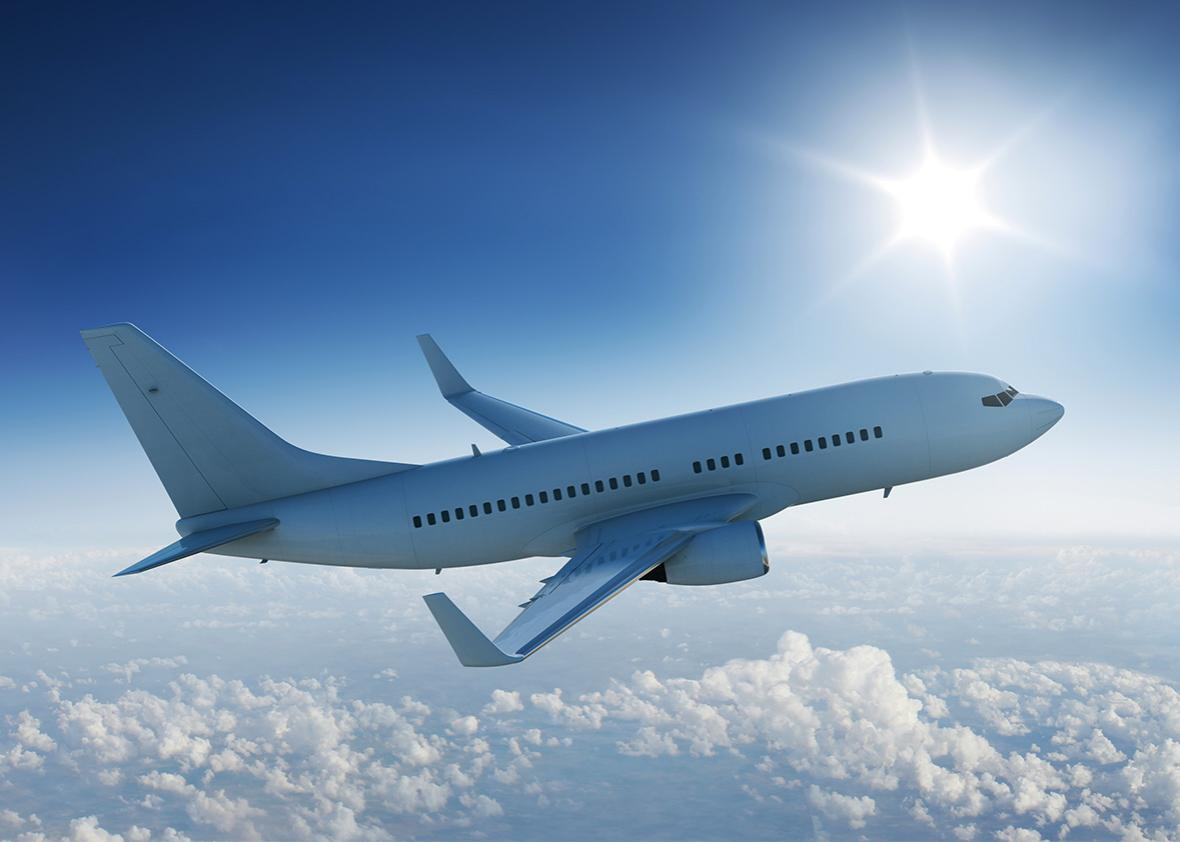
\includegraphics[width=1\linewidth]{Figuras/Ch11/fig1}
	\end{minipage}
	\hfill
	\begin{minipage}{0.49\linewidth}
		\centering
		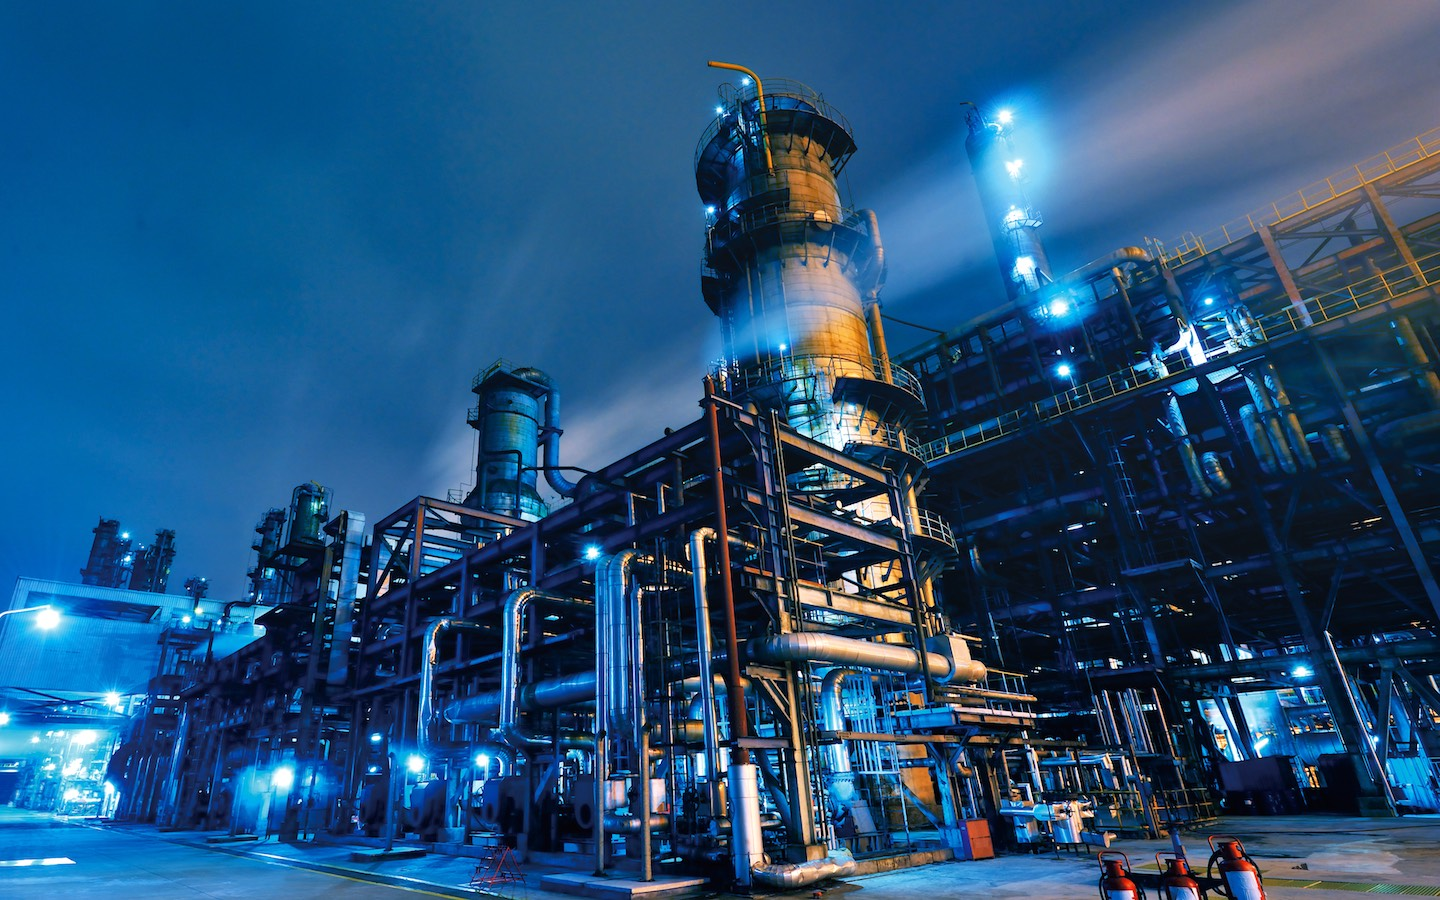
\includegraphics[width=1\linewidth]{Figuras/Ch11/fig2}
	\end{minipage}
\end{frame}


\begin{frame}{Estabilidade}
	\begin{block}{O que é estabilidade?}
		\begin{itemize}
			\item A estabilidade é a medida da facilidade que um processo tem de retornar a um ponto de equilíbrio.
		\end{itemize}
	\end{block}

	\vspace{0.5cm}
	
	\begin{minipage}{0.49\linewidth}
		\centering
		\scalebox{1}{\begin{tikzpicture}[scale=0.5]
			\draw (-4,-3) rectangle (4,3); %CLP
		\draw (-4,0) -- (-2.5,0); %Div in out
		\draw (-2.5,-3) -- (-2.5,3); %Div cartoes
		\draw (-1.5,-2.5) rectangle (0,2.5); %Mem dados
		\draw (0.5,-2.5) rectangle (3.5,-1); %Mem prog
		\draw (1,0) rectangle (3,2); %CPU
		\draw (-4,-5) rectangle (4,-3); %Alimentacao
		\draw (-2.5,4) rectangle (4,6); %Term de prog
		
		\draw (1,2.6) node {CLP};
		
		\draw (-3.25,1.5) node[text width=1.5cm,align=center,rotate=90] {\small Cartões de input};
		
		\draw (-3.25,-1.5) node[text width=1.5cm,align=center,rotate=90] {\small Cartões de output};
		
		\node at (2,1) {\small CPU};
		
		\node[rotate=90,text width=1.5cm,align=center] at (-0.75,0) {\small Memória de dados};
		
		\node[text width=2cm,align=center] at (2,-1.75) {\footnotesize Memória de programa};
		
		\node at (-6,0) {Campo};
		
		\node at (0,-4) {Alimentação};
		
		\node[text width=3cm,align=center] at (0.75,5) {Terminal de programação};
		
		\draw[-Latex] (-8,1.5) -- node[above] {Entradas} +(4,0);
		\draw[Latex-] (-8,-1.5) -- node[below] {Saídas} +(4,0);
		\draw[-Latex] (-2.5,1.5) -- +(1,0);
		\draw[Latex-] (-2.5,-1.5) -- +(1,0);
		\draw[-Latex] (0,1.5) -- +(1,0);
		\draw[Latex-] (0,0.5) -- +(1,0);
		\draw[Latex-] (2,0) -- +(0,-1);
		
		\draw[-Latex] (-1.5,4) -- +(0,-1);
		\draw[Latex-] (3,4) -- +(0,-1);
	\end{tikzpicture}}
	\end{minipage}
	\hfill
	\begin{minipage}{0.49\linewidth}
		\centering
		\scalebox{1}{\newcommand{\innercolor}{gray!70!white}
	\newcommand{\outercolor}{gray!40!white}
	\newcommand{\leftcoil}{red!75!gray}
	\pgfmathsetmacro{\coilseparation}{0.02}
	
	\pgfmathsetmacro{\halflinewidth}{0.008}
	
	
	\begin{tikzpicture}[x={(\xx*1cm,\xy*1cm)},y={(\yx*1cm,\yy*1cm)},z={(\zx*1cm,\zy*1cm)}]
	\draw[\leftcoil, thick] (-0.02,5,1.125) -- +(0,2,0) (1.02,5,3.875) -- +(0,2,0);
	
	\draw[dashed,<->] ($ (-0.02,5,1.125)+(0,2,0) $) -- ($ (1.02,5,3.875)+(0,2,0) $);
	\node[rotate=85] at ($ (-0.02,5+2,1.125)!0.5!(1.02,5+2,3.875)+(0,0.2,0) $) {$ V_p $};
	
	\draw[-latex] (-0.02,6.5,1.325) -- node[above] {$ i_p $} +(0,-1,0);
	\draw[latex-] (1.02,0.02-0.5,1.3) -- node[above] {$ i_s $} +(0,-1,0);
	
	\filldraw[fill=\innercolor]  (0,1,1) -- (1,1,1) -- (1,4,1) -- (0,4,1) -- cycle;
	\filldraw[fill=\innercolor]  (1,4,1) -- (0,4,1) -- (0,4,4) -- (1,4,4) -- cycle;
	\filldraw[fill=\innercolor]  (0,0,0) -- (1,0,0) -- (1,0,5) -- (0,0,5) -- cycle;
	\filldraw[fill=\innercolor]  (0,0,5) -- (0,5,5) -- (1,5,5) -- (1,0,5) -- cycle;
	\filldraw[fill=\outercolor,even odd rule]    (0,0,0) -- (0,5,0) -- (0,5,5) -- (0,0,5) --cycle (0,1,1) -- (0,4,1) -- (0,4,4) -- (0,1,4) --cycle ;
	
	\begin{scope}
	\clip (0,3,1) -- (0,6,1) -- (0,6,4) -- (0,3,4);
	\foreach \z in {1.125,1.375,...,3.875}
	{   \draw[\leftcoil,thick] (0,5,\z) -- (-\coilseparation,5,\z) -- (-\coilseparation,4-\coilseparation,\z) -- (1+\coilseparation,4-\coilseparation,\z) -- (1+\coilseparation,4,\z);
	}
	\end{scope}
	
	
	\foreach \z in {1.25,1.75,...,3.75}
	{   \draw[blue,thick] (0,1,\z) -- (-\coilseparation,1,\z) -- (-\coilseparation,0-\coilseparation,\z) -- (1+\coilseparation,0-\coilseparation,\z) -- (1+\coilseparation,0,\z);
	}

	\draw[blue,thick] (1+\coilseparation,0+\coilseparation,1.1) -- +(0,-2,0) (-\coilseparation,1+\coilseparation,3.85) -- +(0,-3,0);
	
	\draw[dashed,<->] (1.02,-2+0.02,1.1) -- (-0.02,0.02-2,3.85);
	\node[rotate=-70] at ($ (1.02,-2+0.02,1.1)!0.5!(-0.02,0.02-2,3.85)+(0,-0.2,0) $) {$ V_s $};
	
	\draw[decorate,decoration={brace,amplitude=10pt},xshift=-4pt,yshift=0pt] (0,5,1.25) -- +(0,0,2.75);
	\draw[decorate,decoration={brace,amplitude=10pt},xshift=-4pt,yshift=0pt] (1.2,0,3.75) -- +(0,0,-2.6);
	\node[rotate=90] at (0,5.7,2.625) {$ N_p $ espiras};
	\node[rotate=-90] at (1.2,-0.5,2.5) {$ N_s $ espiras};
	
	\draw[dashed,postaction={decorate,decoration={markings,mark=between positions 0.1 and 1 step 0.2 with \arrow{Latex}}}] (0,4.5,0.5) -- (0,0.5,0.5) -- ++(0,0,4) -- ++(0,4,0) -- cycle;
	
	\draw[] (0,2.5,4.7)% -- +(0,-0.5,1.5)
	node[rotate=-10] {Fluxo magnético ($ \phi $)};
	
	\end{tikzpicture}}
	\end{minipage}

	\vspace{0.5cm}

	\centering
	
	\Large	
	Sistema estável
\end{frame}


\begin{frame}{Estabilidade}
	\begin{minipage}{0.49\linewidth}
		\centering
		\scalebox{1}{

\tikzset{every picture/.style={line width=0.75pt}} %set default line width to 0.75pt        

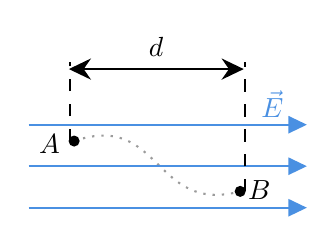
\begin{tikzpicture}[x=0.75pt,y=0.75pt,yscale=-1,xscale=1]
%uncomment if require: \path (0,300); %set diagram left start at 0, and has height of 300

%Curve Lines [id:da6177490068384819] 
\draw [color={rgb, 255:red, 155; green, 155; blue, 155 }  ,draw opacity=1 ] [dash pattern={on 0.84pt off 2.51pt}]  (137.88,127.88) .. controls (180,113.4) and (176,163.4) .. (217.88,152.13) ;


%Straight Lines [id:da7124330895115376] 
\draw [color={rgb, 255:red, 74; green, 144; blue, 226 }  ,draw opacity=1 ]   (116,120) -- (247,120) ;
\draw [shift={(250,120)}, rotate = 180] [fill={rgb, 255:red, 74; green, 144; blue, 226 }  ,fill opacity=1 ][line width=0.08]  [draw opacity=0] (8.93,-4.29) -- (0,0) -- (8.93,4.29) -- cycle    ;

%Straight Lines [id:da12792354611605283] 
\draw [color={rgb, 255:red, 74; green, 144; blue, 226 }  ,draw opacity=1 ]   (116,140) -- (247,140) ;
\draw [shift={(250,140)}, rotate = 180] [fill={rgb, 255:red, 74; green, 144; blue, 226 }  ,fill opacity=1 ][line width=0.08]  [draw opacity=0] (8.93,-4.29) -- (0,0) -- (8.93,4.29) -- cycle    ;

%Straight Lines [id:da4044562129660001] 
\draw [color={rgb, 255:red, 74; green, 144; blue, 226 }  ,draw opacity=1 ]   (116,160) -- (247,160) ;
\draw [shift={(250,160)}, rotate = 180] [fill={rgb, 255:red, 74; green, 144; blue, 226 }  ,fill opacity=1 ][line width=0.08]  [draw opacity=0] (8.93,-4.29) -- (0,0) -- (8.93,4.29) -- cycle    ;

%Shape: Circle [id:dp28224868607946574] 
\draw  [fill={rgb, 255:red, 0; green, 0; blue, 0 }  ,fill opacity=1 ] (135.75,127.88) .. controls (135.75,126.7) and (136.7,125.75) .. (137.88,125.75) .. controls (139.05,125.75) and (140,126.7) .. (140,127.88) .. controls (140,129.05) and (139.05,130) .. (137.88,130) .. controls (136.7,130) and (135.75,129.05) .. (135.75,127.88) -- cycle ;
%Shape: Circle [id:dp03942976292609046] 
\draw  [color={rgb, 255:red, 0; green, 0; blue, 0 }  ,draw opacity=1 ][fill={rgb, 255:red, 0; green, 0; blue, 0 }  ,fill opacity=1 ] (215.75,152.13) .. controls (215.75,150.95) and (216.7,150) .. (217.88,150) .. controls (219.05,150) and (220,150.95) .. (220,152.13) .. controls (220,153.3) and (219.05,154.25) .. (217.88,154.25) .. controls (216.7,154.25) and (215.75,153.3) .. (215.75,152.13) -- cycle ;
%Straight Lines [id:da5788684610773114] 
\draw  [dash pattern={on 4.5pt off 4.5pt}]  (135.75,127.88) -- (135.75,90) ;


%Straight Lines [id:da7063621547892809] 
\draw  [dash pattern={on 4.5pt off 4.5pt}]  (220,152.13) -- (220,90) ;


%Straight Lines [id:da8063380246624134] 
\draw    (138.35,93.2) -- (216.6,93.2) ;
\draw [shift={(219.6,93.2)}, rotate = 180] [fill={rgb, 255:red, 0; green, 0; blue, 0 }  ][line width=0.08]  [draw opacity=0] (10.72,-5.15) -- (0,0) -- (10.72,5.15) -- (7.12,0) -- cycle    ;
\draw [shift={(135.35,93.2)}, rotate = 0] [fill={rgb, 255:red, 0; green, 0; blue, 0 }  ][line width=0.08]  [draw opacity=0] (10.72,-5.15) -- (0,0) -- (10.72,5.15) -- (7.12,0) -- cycle    ;

% Text Node
\draw (233.4,110) node [color={rgb, 255:red, 74; green, 144; blue, 226 }  ,opacity=1 ]  {$\vec{E}$};
% Text Node
\draw (177.33,82.33) node   {$d$};
% Text Node
\draw (126,129.33) node   {$A$};
% Text Node
\draw (227.13,151.4) node   {$B$};


\end{tikzpicture}
}
	\end{minipage}
	\hfill
	\begin{minipage}{0.49\linewidth}
		\centering
		
		\vspace{-0.7cm}
		\scalebox{1}{

\tikzset{every picture/.style={line width=0.75pt}} %set default line width to 0.75pt        

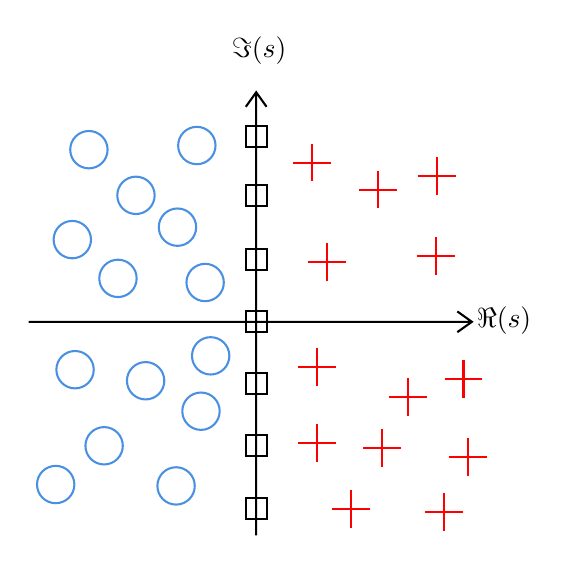
\begin{tikzpicture}[x=0.75pt,y=0.75pt,yscale=-1,xscale=1]
%uncomment if require: \path (0,300); %set diagram left start at 0, and has height of 300

%Shape: Axis 2D [id:dp27678030181731494] 
\draw  (40,160.6) -- (253.5,160.6)(149.6,50) -- (149.6,263.5) (246.5,155.6) -- (253.5,160.6) -- (246.5,165.6) (144.6,57) -- (149.6,50) -- (154.6,57)  ;
%Shape: Square [id:dp29640104318485094] 
\draw   (144.6,155.6) -- (154.6,155.6) -- (154.6,165.6) -- (144.6,165.6) -- cycle ;
%Shape: Square [id:dp5015049228757054] 
\draw   (144.6,125.7) -- (154.6,125.7) -- (154.6,135.7) -- (144.6,135.7) -- cycle ;
%Shape: Square [id:dp5724308304859749] 
\draw   (144.6,94.7) -- (154.6,94.7) -- (154.6,104.7) -- (144.6,104.7) -- cycle ;
%Shape: Square [id:dp8722658997981245] 
\draw   (144.6,66.2) -- (154.6,66.2) -- (154.6,76.2) -- (144.6,76.2) -- cycle ;
%Shape: Square [id:dp035501458242915174] 
\draw   (144.6,185.2) -- (154.6,185.2) -- (154.6,195.2) -- (144.6,195.2) -- cycle ;
%Shape: Square [id:dp23226558696093957] 
\draw   (144.6,215.2) -- (154.6,215.2) -- (154.6,225.2) -- (144.6,225.2) -- cycle ;
%Shape: Square [id:dp09667812864869552] 
\draw   (144.6,245.7) -- (154.6,245.7) -- (154.6,255.7) -- (144.6,255.7) -- cycle ;
\draw  [color={rgb, 255:red, 255; green, 0; blue, 0 }  ,draw opacity=1 ] (167.5,83.88) -- (185.75,83.88)(176.63,74.75) -- (176.63,93) ;
\draw  [color={rgb, 255:red, 255; green, 0; blue, 0 }  ,draw opacity=1 ] (199,96.88) -- (217.25,96.88)(208.13,87.75) -- (208.13,106) ;
\draw  [color={rgb, 255:red, 255; green, 0; blue, 0 }  ,draw opacity=1 ] (174.5,131.88) -- (192.75,131.88)(183.63,122.75) -- (183.63,141) ;
\draw  [color={rgb, 255:red, 255; green, 0; blue, 0 }  ,draw opacity=1 ] (227,128.88) -- (245.25,128.88)(236.13,119.75) -- (236.13,138) ;
\draw  [color={rgb, 255:red, 255; green, 0; blue, 0 }  ,draw opacity=1 ] (227.5,90.38) -- (245.75,90.38)(236.63,81.25) -- (236.63,99.5) ;
\draw  [color={rgb, 255:red, 255; green, 0; blue, 0 }  ,draw opacity=1 ] (169.67,182.21) -- (187.92,182.21)(178.79,173.08) -- (178.79,191.33) ;
\draw  [color={rgb, 255:red, 255; green, 0; blue, 0 }  ,draw opacity=1 ] (186.33,250.88) -- (204.58,250.88)(195.46,241.75) -- (195.46,260) ;
\draw  [color={rgb, 255:red, 255; green, 0; blue, 0 }  ,draw opacity=1 ] (231,252.21) -- (249.25,252.21)(240.13,243.08) -- (240.13,261.33) ;
\draw  [color={rgb, 255:red, 255; green, 0; blue, 0 }  ,draw opacity=1 ] (169.67,218.88) -- (187.92,218.88)(178.79,209.75) -- (178.79,228) ;
\draw  [color={rgb, 255:red, 255; green, 0; blue, 0 }  ,draw opacity=1 ] (242.33,225.54) -- (260.58,225.54)(251.46,216.42) -- (251.46,234.67) ;
\draw  [color={rgb, 255:red, 255; green, 0; blue, 0 }  ,draw opacity=1 ] (213.67,196.88) -- (231.92,196.88)(222.79,187.75) -- (222.79,206) ;
\draw  [color={rgb, 255:red, 255; green, 0; blue, 0 }  ,draw opacity=1 ] (240.33,188.21) -- (258.58,188.21)(249.46,179.08) -- (249.46,197.33) ;
\draw  [color={rgb, 255:red, 255; green, 0; blue, 0 }  ,draw opacity=1 ] (201,221.54) -- (219.25,221.54)(210.13,212.42) -- (210.13,230.67) ;
%Shape: Circle [id:dp01739200493370019] 
\draw  [color={rgb, 255:red, 74; green, 144; blue, 226 }  ,draw opacity=1 ] (60,77.67) .. controls (60,72.7) and (64.03,68.67) .. (69,68.67) .. controls (73.97,68.67) and (78,72.7) .. (78,77.67) .. controls (78,82.64) and (73.97,86.67) .. (69,86.67) .. controls (64.03,86.67) and (60,82.64) .. (60,77.67) -- cycle ;
%Shape: Circle [id:dp857755141402053] 
\draw  [color={rgb, 255:red, 74; green, 144; blue, 226 }  ,draw opacity=1 ] (82.67,99.67) .. controls (82.67,94.7) and (86.7,90.67) .. (91.67,90.67) .. controls (96.64,90.67) and (100.67,94.7) .. (100.67,99.67) .. controls (100.67,104.64) and (96.64,108.67) .. (91.67,108.67) .. controls (86.7,108.67) and (82.67,104.64) .. (82.67,99.67) -- cycle ;
%Shape: Circle [id:dp9246833060771249] 
\draw  [color={rgb, 255:red, 74; green, 144; blue, 226 }  ,draw opacity=1 ] (44,239) .. controls (44,234.03) and (48.03,230) .. (53,230) .. controls (57.97,230) and (62,234.03) .. (62,239) .. controls (62,243.97) and (57.97,248) .. (53,248) .. controls (48.03,248) and (44,243.97) .. (44,239) -- cycle ;
%Shape: Circle [id:dp8304441936419562] 
\draw  [color={rgb, 255:red, 74; green, 144; blue, 226 }  ,draw opacity=1 ] (118.67,177) .. controls (118.67,172.03) and (122.7,168) .. (127.67,168) .. controls (132.64,168) and (136.67,172.03) .. (136.67,177) .. controls (136.67,181.97) and (132.64,186) .. (127.67,186) .. controls (122.7,186) and (118.67,181.97) .. (118.67,177) -- cycle ;
%Shape: Circle [id:dp5059258663614863] 
\draw  [color={rgb, 255:red, 74; green, 144; blue, 226 }  ,draw opacity=1 ] (102.67,115) .. controls (102.67,110.03) and (106.7,106) .. (111.67,106) .. controls (116.64,106) and (120.67,110.03) .. (120.67,115) .. controls (120.67,119.97) and (116.64,124) .. (111.67,124) .. controls (106.7,124) and (102.67,119.97) .. (102.67,115) -- cycle ;
%Shape: Circle [id:dp21245040687156935] 
\draw  [color={rgb, 255:red, 74; green, 144; blue, 226 }  ,draw opacity=1 ] (52,121) .. controls (52,116.03) and (56.03,112) .. (61,112) .. controls (65.97,112) and (70,116.03) .. (70,121) .. controls (70,125.97) and (65.97,130) .. (61,130) .. controls (56.03,130) and (52,125.97) .. (52,121) -- cycle ;
%Shape: Circle [id:dp17429736806925722] 
\draw  [color={rgb, 255:red, 74; green, 144; blue, 226 }  ,draw opacity=1 ] (116,141.67) .. controls (116,136.7) and (120.03,132.67) .. (125,132.67) .. controls (129.97,132.67) and (134,136.7) .. (134,141.67) .. controls (134,146.64) and (129.97,150.67) .. (125,150.67) .. controls (120.03,150.67) and (116,146.64) .. (116,141.67) -- cycle ;
%Shape: Circle [id:dp33160849295458217] 
\draw  [color={rgb, 255:red, 74; green, 144; blue, 226 }  ,draw opacity=1 ] (74,139.67) .. controls (74,134.7) and (78.03,130.67) .. (83,130.67) .. controls (87.97,130.67) and (92,134.7) .. (92,139.67) .. controls (92,144.64) and (87.97,148.67) .. (83,148.67) .. controls (78.03,148.67) and (74,144.64) .. (74,139.67) -- cycle ;
%Shape: Circle [id:dp32709834546378724] 
\draw  [color={rgb, 255:red, 74; green, 144; blue, 226 }  ,draw opacity=1 ] (87.33,189) .. controls (87.33,184.03) and (91.36,180) .. (96.33,180) .. controls (101.3,180) and (105.33,184.03) .. (105.33,189) .. controls (105.33,193.97) and (101.3,198) .. (96.33,198) .. controls (91.36,198) and (87.33,193.97) .. (87.33,189) -- cycle ;
%Shape: Circle [id:dp8791724327388495] 
\draw  [color={rgb, 255:red, 74; green, 144; blue, 226 }  ,draw opacity=1 ] (53.33,183.67) .. controls (53.33,178.7) and (57.36,174.67) .. (62.33,174.67) .. controls (67.3,174.67) and (71.33,178.7) .. (71.33,183.67) .. controls (71.33,188.64) and (67.3,192.67) .. (62.33,192.67) .. controls (57.36,192.67) and (53.33,188.64) .. (53.33,183.67) -- cycle ;
%Shape: Circle [id:dp4794866171308949] 
\draw  [color={rgb, 255:red, 74; green, 144; blue, 226 }  ,draw opacity=1 ] (114,203.67) .. controls (114,198.7) and (118.03,194.67) .. (123,194.67) .. controls (127.97,194.67) and (132,198.7) .. (132,203.67) .. controls (132,208.64) and (127.97,212.67) .. (123,212.67) .. controls (118.03,212.67) and (114,208.64) .. (114,203.67) -- cycle ;
%Shape: Circle [id:dp5349657045143856] 
\draw  [color={rgb, 255:red, 74; green, 144; blue, 226 }  ,draw opacity=1 ] (67.33,220.33) .. controls (67.33,215.36) and (71.36,211.33) .. (76.33,211.33) .. controls (81.3,211.33) and (85.33,215.36) .. (85.33,220.33) .. controls (85.33,225.3) and (81.3,229.33) .. (76.33,229.33) .. controls (71.36,229.33) and (67.33,225.3) .. (67.33,220.33) -- cycle ;
%Shape: Circle [id:dp714149478603834] 
\draw  [color={rgb, 255:red, 74; green, 144; blue, 226 }  ,draw opacity=1 ] (102,239.67) .. controls (102,234.7) and (106.03,230.67) .. (111,230.67) .. controls (115.97,230.67) and (120,234.7) .. (120,239.67) .. controls (120,244.64) and (115.97,248.67) .. (111,248.67) .. controls (106.03,248.67) and (102,244.64) .. (102,239.67) -- cycle ;
%Shape: Circle [id:dp476022910470574] 
\draw  [color={rgb, 255:red, 74; green, 144; blue, 226 }  ,draw opacity=1 ] (112,75.67) .. controls (112,70.7) and (116.03,66.67) .. (121,66.67) .. controls (125.97,66.67) and (130,70.7) .. (130,75.67) .. controls (130,80.64) and (125.97,84.67) .. (121,84.67) .. controls (116.03,84.67) and (112,80.64) .. (112,75.67) -- cycle ;

% Text Node
\draw (151,30) node   {$\Im(s)$};
% Text Node
\draw (269,160) node   {$\Re(s)$};


\end{tikzpicture}}
	\end{minipage}

	\vspace{1cm}

	\centering

	\Large
	Sistema instável
\end{frame}


\begin{frame}{Estabilidade}
	\begin{minipage}{0.49\linewidth}
		\centering
		\scalebox{0.8}{

\tikzset{every picture/.style={line width=0.75pt}} %set default line width to 0.75pt        

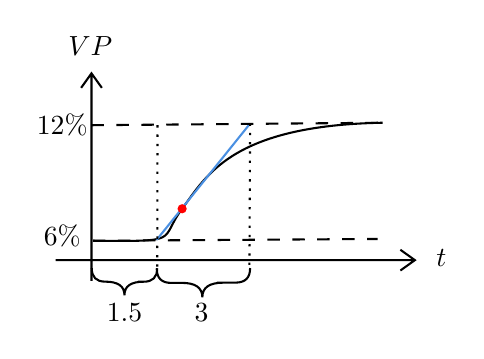
\begin{tikzpicture}[x=0.75pt,y=0.75pt,yscale=-1,xscale=1]
%uncomment if require: \path (0,300); %set diagram left start at 0, and has height of 300

%Shape: Axis 2D [id:dp8434144691544803] 
\draw  (61.27,196) -- (234.4,196)(78.58,106) -- (78.58,206) (227.4,191) -- (234.4,196) -- (227.4,201) (73.58,113) -- (78.58,106) -- (83.58,113)  ;
%Curve Lines [id:da3393494842698659] 
\draw    (79.33,186.67) .. controls (123.2,187) and (110.65,186.84) .. (122.25,171.24) .. controls (133.85,155.64) and (145.88,131.07) .. (218.8,129.8) ;


%Straight Lines [id:da773558557641419] 
\draw [color={rgb, 255:red, 74; green, 144; blue, 226 }  ,draw opacity=1 ]   (155,130.2) -- (110,186.2) ;


%Shape: Circle [id:dp28048312241562945] 
\draw  [color={rgb, 255:red, 255; green, 0; blue, 0 }  ,draw opacity=1 ][fill={rgb, 255:red, 255; green, 0; blue, 0 }  ,fill opacity=1 ] (120.58,171.24) .. controls (120.58,170.32) and (121.33,169.57) .. (122.25,169.57) .. controls (123.17,169.57) and (123.92,170.32) .. (123.92,171.24) .. controls (123.92,172.16) and (123.17,172.91) .. (122.25,172.91) .. controls (121.33,172.91) and (120.58,172.16) .. (120.58,171.24) -- cycle ;
%Straight Lines [id:da6828905031101673] 
\draw  [dash pattern={on 4.5pt off 4.5pt}]  (78.6,131) -- (218.8,129.8) ;


%Straight Lines [id:da012395283086218845] 
\draw  [dash pattern={on 4.5pt off 4.5pt}]  (79.33,186.67) -- (216.4,185.8) ;


%Shape: Brace [id:dp15969553307240192] 
\draw   (78.71,199.86) .. controls (78.7,204.19) and (80.87,206.35) .. (85.2,206.36) -- (85.2,206.36) .. controls (91.38,206.37) and (94.47,208.54) .. (94.46,212.87) .. controls (94.47,208.54) and (97.56,206.38) .. (103.75,206.39)(100.96,206.38) -- (103.75,206.39) .. controls (108.08,206.4) and (110.24,204.24) .. (110.25,199.91) ;
%Shape: Brace [id:dp058145123409859556] 
\draw   (110,200) .. controls (110.02,204.67) and (112.36,206.99) .. (117.03,206.97) -- (121.96,206.95) .. controls (128.63,206.92) and (131.97,209.23) .. (131.99,213.9) .. controls (131.97,209.23) and (135.29,206.89) .. (141.96,206.86)(138.96,206.87) -- (148.03,206.83) .. controls (152.7,206.81) and (155.02,204.47) .. (155,199.8) ;
%Straight Lines [id:da9569907625895342] 
\draw  [dash pattern={on 0.84pt off 2.51pt}]  (155,130.2) -- (154.68,198.45) ;


%Straight Lines [id:da25982411660347404] 
\draw  [dash pattern={on 0.84pt off 2.51pt}]  (110.4,131) -- (110.25,200.52) ;



% Text Node
\draw (247.2,194.8) node   {$t$};
% Text Node
\draw (78,93) node   {$VP$};
% Text Node
\draw (94.53,221.43) node   {$\SI{1.5}{\second}$};
% Text Node
\draw (131.58,221.2) node   {$\SI{3}{\second}$};
% Text Node
\draw (64.5,131) node   {$12\%$};
% Text Node
\draw (64.5,184.5) node   {$6\%$};


\end{tikzpicture}
}
		
		\medskip
		
		Sistema estável
	\end{minipage}
	\hfill
	\begin{minipage}{0.49\linewidth}
		\centering
		
		\vspace{1.6cm}
		\scalebox{1.2}{\begin{tikzpicture}
	\draw[->] (-2.5,0) -- (2.5,0) node[right] {$ \sigma $};
	\draw[->] (0,-2) -- (0,2) node[above] {$ j\omega $};
	
	\draw (0,0) node[below left] {$ 0 $};
	
	\draw (-1,-2) -- (-1,2) (1,-2) -- (1,2);
	
	\node [above left] at (-1,0) {$ -\sigma_1 $};
	\node [above right] at (1,0) {$ \sigma_2 $};
\end{tikzpicture}}
		
		\medskip
		
		Sistema instável
	\end{minipage}
	
	\vspace{1cm}
	
	\centering
	
	\Large
	
\end{frame}


%\begin{frame}{Estabilidade}
%	\begin{block}{BIBO estabilidade}
%		\begin{itemize}
%			\item Um sistema é BIBO (\textit{Bounded-Input, Bounded-Output}) estável se ele possui uma saída que é limitada tal qual sua entrada.
%		\end{itemize}
%	\end{block}
%
%	\vspace{0.3cm}
%	\begin{minipage}{0.49\linewidth}
%		\centering
%		
%		\scalebox{0.9}{

\tikzset{every picture/.style={line width=0.75pt}} %set default line width to 0.75pt        

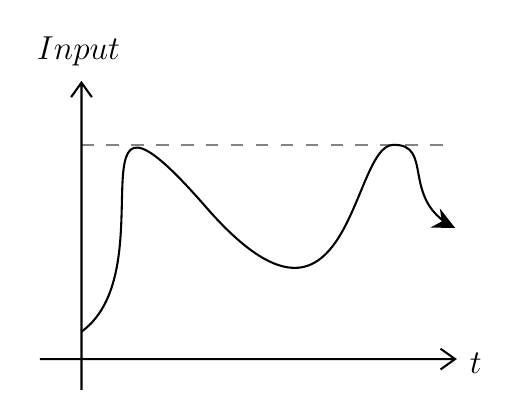
\begin{tikzpicture}[x=0.75pt,y=0.75pt,yscale=-1,xscale=1]
%uncomment if require: \path (0,300); %set diagram left start at 0, and has height of 300

%Straight Lines [id:da26643584263795916] 
\draw [color={rgb, 255:red, 131; green, 131; blue, 131 }  ,draw opacity=1 ] [dash pattern={on 4.5pt off 4.5pt}]  (90,100) -- (270,100) ;


%Shape: Axis 2D [id:dp7046941980103143] 
\draw  (70,203.2) -- (270,203.2)(90,70) -- (90,218) (263,198.2) -- (270,203.2) -- (263,208.2) (85,77) -- (90,70) -- (95,77)  ;
%Curve Lines [id:da03413665677920852] 
\draw    (90,190) .. controls (132.33,159.33) and (80.33,50) .. (150,130) .. controls (219.67,210) and (219.67,100.67) .. (240,100) .. controls (259.93,99.35) and (243.68,125.58) .. (268.43,139.18) ;
\draw [shift={(270,140)}, rotate = 206.28] [fill={rgb, 255:red, 0; green, 0; blue, 0 }  ][line width=0.75]  [draw opacity=0] (10.72,-5.15) -- (0,0) -- (10.72,5.15) -- (7.12,0) -- cycle    ;


% Text Node
\draw (88.5,55) node   {\large $Input$};
% Text Node
\draw (280,205) node   {\large $t$};


\end{tikzpicture}
}
%	\end{minipage}
%	\hfill
%	\begin{minipage}{0.49\linewidth}
%		\centering
%		
%		\scalebox{0.9}{

\tikzset{every picture/.style={line width=0.75pt}} %set default line width to 0.75pt        

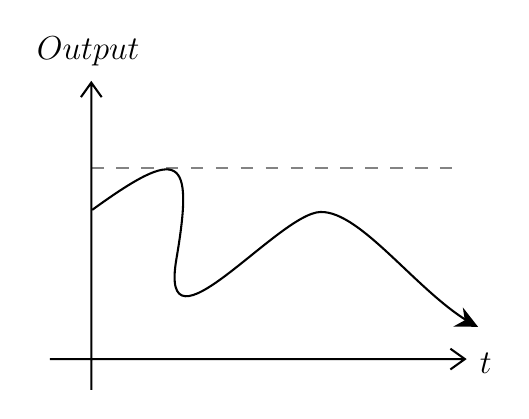
\begin{tikzpicture}[x=0.75pt,y=0.75pt,yscale=-1,xscale=1]
%uncomment if require: \path (0,300); %set diagram left start at 0, and has height of 300

%Straight Lines [id:da45173516768188793] 
\draw [color={rgb, 255:red, 131; green, 131; blue, 131 }  ,draw opacity=1 ] [dash pattern={on 4.5pt off 4.5pt}]  (110,131.33) -- (290,131.33) ;


%Shape: Axis 2D [id:dp17702348361548204] 
\draw  (90,223.2) -- (290,223.2)(110,90) -- (110,238) (283,218.2) -- (290,223.2) -- (283,228.2) (105,97) -- (110,90) -- (115,97)  ;
%Curve Lines [id:da6473783232781454] 
\draw    (110.42,151.33) .. controls (152.75,120.66) and (159.67,124.33) .. (151,174.99) .. controls (142.33,225.66) and (200,152.99) .. (220.33,152.33) .. controls (240.26,151.67) and (268.19,192.64) .. (294.71,206.83) ;
\draw [shift={(296.33,207.66)}, rotate = 206.28] [fill={rgb, 255:red, 0; green, 0; blue, 0 }  ][line width=0.75]  [draw opacity=0] (10.72,-5.15) -- (0,0) -- (10.72,5.15) -- (7.12,0) -- cycle    ;


% Text Node
\draw (108.5,75) node   {\large $Output$};
% Text Node
\draw (300,225) node   {\large $t$};


\end{tikzpicture}
}
%	\end{minipage}
%\end{frame}


\begin{frame}{Conceitos preliminares}
	\begin{block}{Processo}
		\begin{itemize}
			\item Um \textbf{processo} é qualquer atividade (ou conjunto de atividades) que tem algum \textbf{objetivo}.
		\end{itemize}
	\end{block}

	\vspace{0.5cm}

	\begin{minipage}{0.49\linewidth}
		\centering
		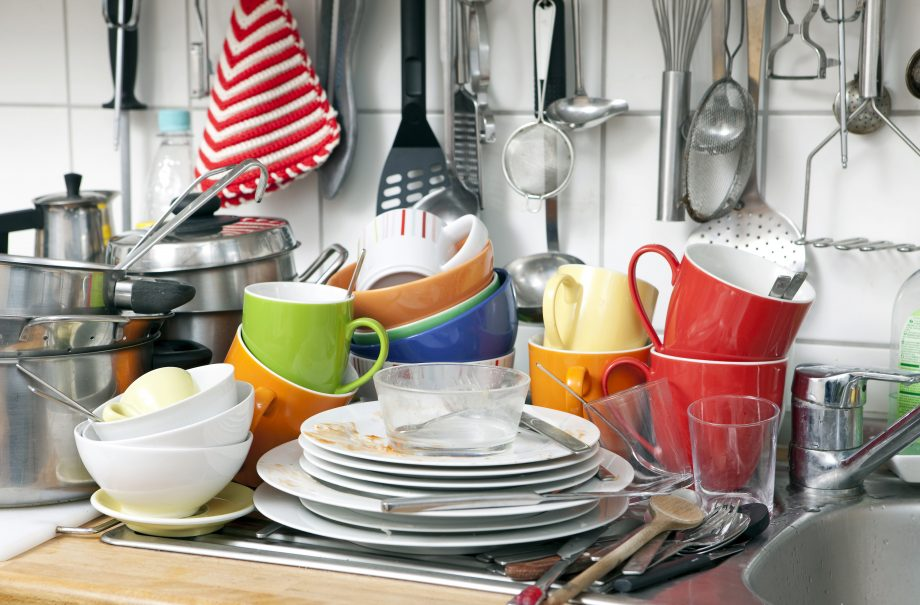
\includegraphics[width=1\linewidth]{Figuras/Ch11/fig3}
	\end{minipage}
	\hfill
	\begin{minipage}{0.49\linewidth}
		\centering
		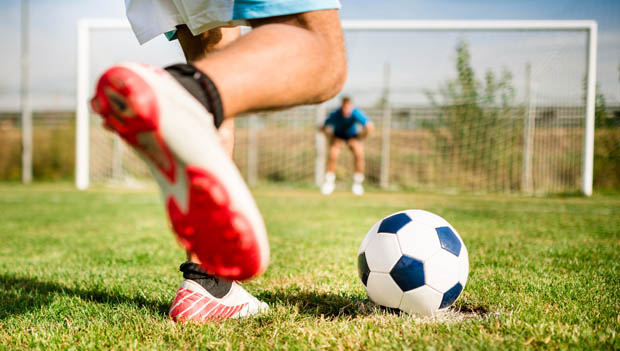
\includegraphics[width=1\linewidth]{Figuras/Ch11/fig4}
	\end{minipage}
\end{frame}


\begin{frame}{Conceitos preliminares}
	\begin{block}{Variáveis de processo}
		\begin{itemize}
			\item As \textbf{variáveis de processo} são aquelas \textbf{envolvidas no processo}.
			\item Estas podem ser alteradas durante o processo, e podem ser usadas para \textbf{medir os resultados} e/ou \textbf{controlá-los}.
		\end{itemize}
	\end{block}
	
%	\vspace{0.5cm}
	
	\centering
	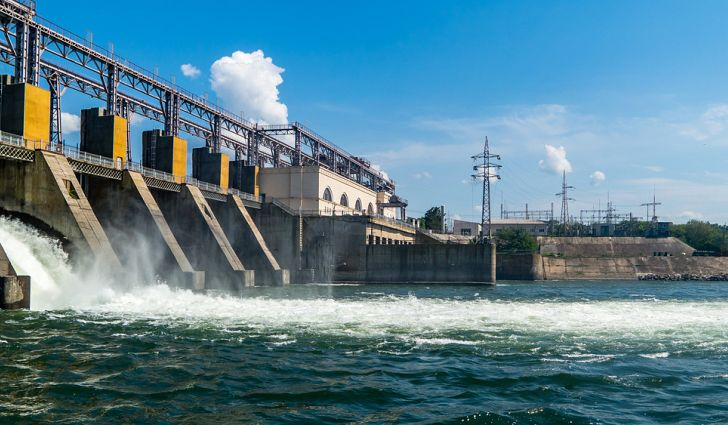
\includegraphics[width=0.8\linewidth]{Figuras/Ch11/fig5}
\end{frame}


\begin{frame}{Conceitos preliminares}
	\begin{block}{Outras variáveis e \textit{setpoint}}
		\begin{itemize}
			\item O \textbf{controle de processos} vai ajustar uma \textbf{variável manipulada} e, assim, estabilizar a \textbf{variável controlada} em seu \textbf{\textit{setpoint}}.
		\end{itemize}
	\end{block}
	
	%	\vspace{0.5cm}
	
	\centering
	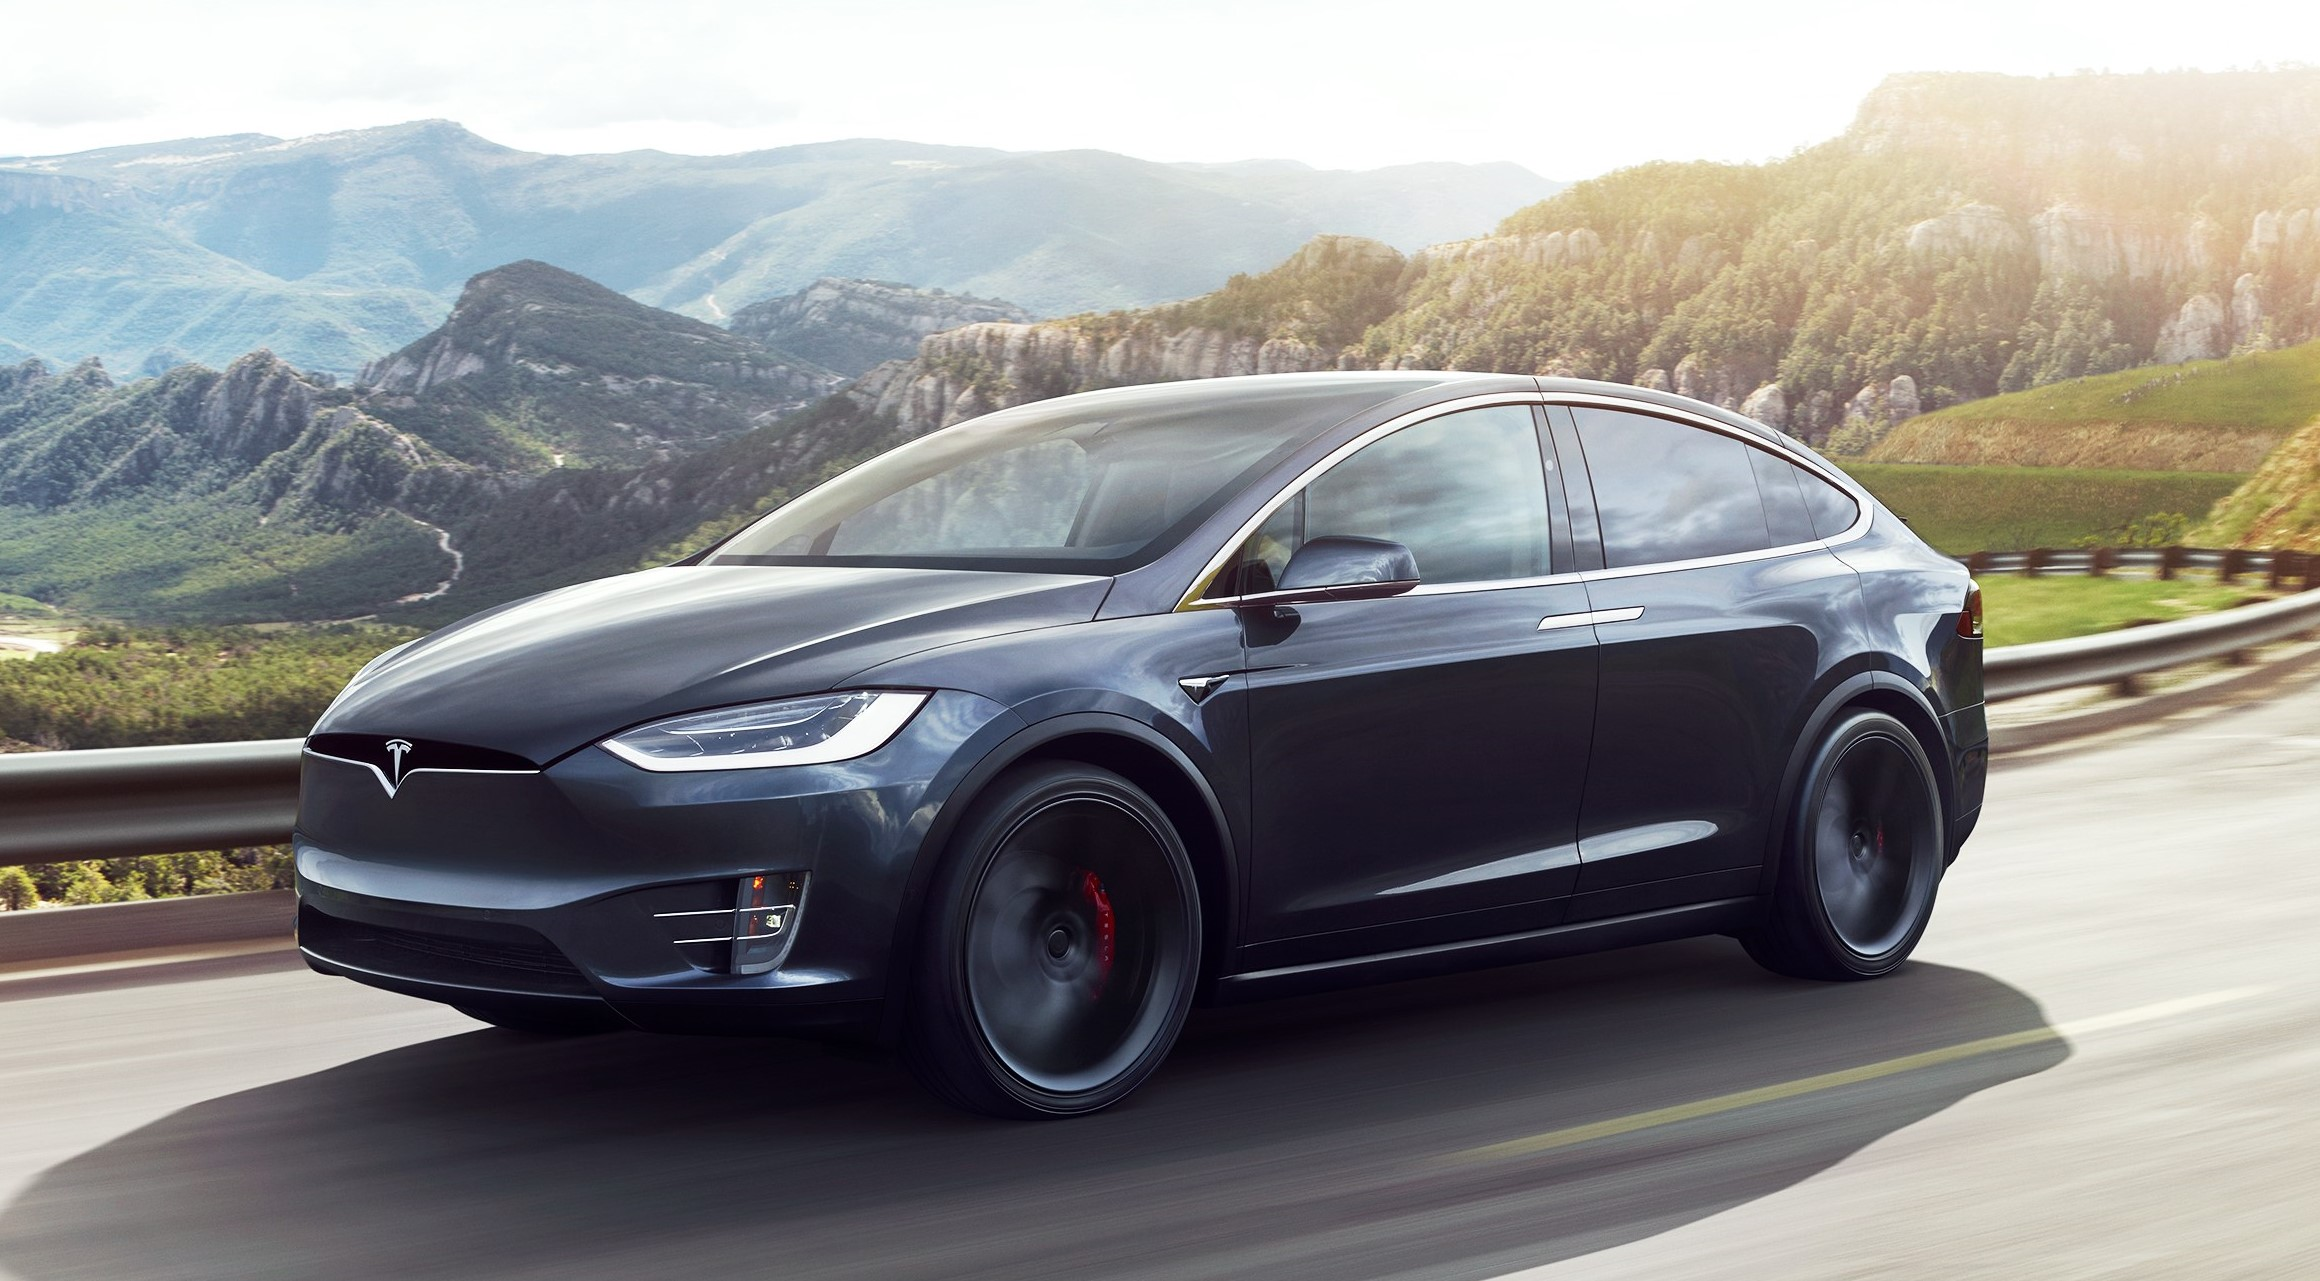
\includegraphics[width=0.8\linewidth]{Figuras/Ch11/fig6}
\end{frame}


\begin{frame}{Malha aberta x malha fechada}
	\begin{block}{Introdução}
		\begin{itemize}
			\item O controle de malha aberta pode ser suficiente em vários sistemas onde as condições de operação são \textbf{constantes}, mas e se não forem?
		\end{itemize}
	\end{block}
	
	%	\vspace{0.5cm}
	
	\centering
	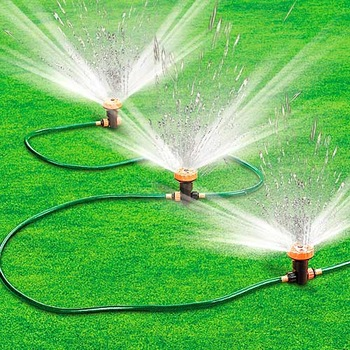
\includegraphics[height=0.65\textheight]{Figuras/Ch11/fig7}
\end{frame}


\begin{frame}{Malha aberta x malha fechada}
	\begin{block}{Diagramas de blocos}
		\begin{itemize}
			\item Os diagramas de blocos nos ajudam a compreender o funcionamento das malhas, indicando cada componente e sua função na malha.
		\end{itemize}
	\end{block}
	
	\vspace{1cm}
	
	\centering
	\deftkzbds
	\begin{tikzpicture}[auto, node distance=2cm,>=Latex]
	\node[input] (in) {};
	\node[block, right=of in] (B) {Bloco};
	\node[output,right=of B] (out) {}; 
	
	\draw[->] (in) -- node[above,midway] {Entrada} (B);
	\draw[->] (B) -- node[above,midway] {Saída} (out);
	\end{tikzpicture}
\end{frame}


\begin{frame}{Malha aberta x malha fechada}
	\begin{block}{Malha aberta}
		\begin{itemize}
			\item Uma \textbf{malha aberta} pode ser mostrada por um diagrama de blocos com apenas dois elementos.
			\item A malha aberta pode lidar com \textbf{quaisquer problemas já conhecidos}, pois já são contados em seu \textbf{funcionamento normal}.
		\end{itemize}
	\end{block}
	
	\vspace{1cm}
	
	\centering
	\deftkzbds
	\begin{tikzpicture}[auto, node distance=2cm,>=Latex]
	\node[input] (in) {};
	\node[block, right=of in] (C) {Controlador};
	\node[block, right=of C] (P) {Processo};
	\node[output,right=of P] (out) {}; 
	
	\draw[->] (in) -- node[above,midway] {Entrada} (C);
	\draw[->] (C) -- (P);
	\draw[->] (P) -- (out) node[above,midway] {Saída};
	\end{tikzpicture}
\end{frame}


\begin{frame}{Malha aberta x malha fechada}
	\begin{block}{Malha fechada}
		A malha fechada conta com alguns componentes adicionais, entre eles:
		\begin{itemize}
			\item \textbf{Comparador}
			
			Compara o valor de \textbf{referência} com o \textbf{valor medido} na saída e gera um sinal de \textbf{erro} que indica o quanto o sinal de saída está longe do sinal de entrada.
			\item \textbf{Atuador}
			
			A partir do sinal recebido do controlador, atua sobre a \textbf{variável manipulada} para ajustar e alterar a variável controlada de modo a \textbf{corrigir o erro}.
			\item \textbf{Sensor}
			
			\textbf{Lê a variável controlada} na saída e envia sua condição na forma de sinal para o comparador, fechando o laço.
		\end{itemize}
	\end{block}
\end{frame}


\begin{frame}{Malha aberta x malha fechada}
	\begin{block}{Malha fechada}
		\begin{itemize}
			\item Os componentes da malha fechada devem regular sua saída \textbf{independentemente} das condições do processo.
			\item O sensor deverá \textbf{ler a saída} e \textbf{enviar seu sinal} (através de um transmissor) para o comparador, que deve enviar o \textbf{erro} para o controlador.
			\item O controlador, então, deve enviar um sinal calculado (ao atuador) para \textbf{corrigir} a saída do processo, que deve tender ao \textbf{valor desejado} (\textit{setpoint}).
		\end{itemize}
	\end{block}

%	\vspace{0.5cm}
	
	\centering
	\scalebox{0.7}{
		\deftkzbds
		\begin{tikzpicture}[auto, node distance=1cm,>=Latex]
			\node[input] (in) {};
			\node[sum,right=1.5cm of in] (sum) {\Large $ + $};
			\node[block, right=of sum] (C) {Controlador};
			\node[block,right=of C] (A) {Atuador};
			\node[block, right=of A] (P) {Processo};
			\coordinate[right=of P] (mid);
			\node[output,right=of mid] (out) {};
			\node[block,below=of A] (S) {Sensor};
			
			\draw[->] (in) -- node[above,midway] {Entrada} (sum) node[above=12pt] {Comparador};
			\draw[->] (sum) -- (C);
			\draw[->] (C) -- (A);
			\draw[->] (A) -- (P);
			\draw[->] (mid) |- (S);
			\draw[->] (S) -| node[pos=0.98, xshift=15pt] {$-$} node[pos=1.19, xshift=-4pt] {$+$} (sum);
			\draw[->] (P) -- (out) node[above,near end] {Saída};
		\end{tikzpicture}}
\end{frame}


\begin{frame}{Correção da saída}
	\begin{block}{Introdução}
		\begin{itemize}
			\item Assim que é detectada uma \textbf{anormalidade} na saída, isto é, um \textbf{erro}, em uma malha fechada, o controlador deve responder para corrigí-lo.
			\item Se o erro for \textbf{muito grande}, a resposta do controlador pode ser \textbf{muito drástica}, causando um erro \textbf{tão grande quanto}, mas \textbf{oposto} ao original.
		\end{itemize}
	\end{block}

	\vspace{-1.5cm}

	\centering
	\scalebox{0.8}{

\tikzset{every picture/.style={line width=0.75pt}} %set default line width to 0.75pt        

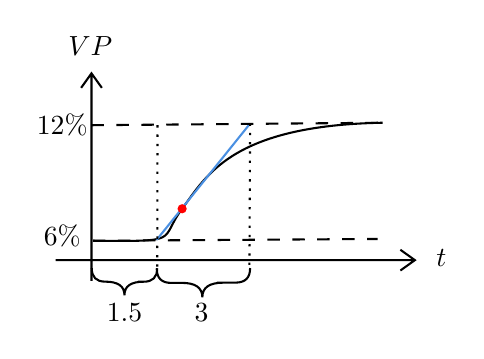
\begin{tikzpicture}[x=0.75pt,y=0.75pt,yscale=-1,xscale=1]
%uncomment if require: \path (0,300); %set diagram left start at 0, and has height of 300

%Shape: Axis 2D [id:dp8434144691544803] 
\draw  (61.27,196) -- (234.4,196)(78.58,106) -- (78.58,206) (227.4,191) -- (234.4,196) -- (227.4,201) (73.58,113) -- (78.58,106) -- (83.58,113)  ;
%Curve Lines [id:da3393494842698659] 
\draw    (79.33,186.67) .. controls (123.2,187) and (110.65,186.84) .. (122.25,171.24) .. controls (133.85,155.64) and (145.88,131.07) .. (218.8,129.8) ;


%Straight Lines [id:da773558557641419] 
\draw [color={rgb, 255:red, 74; green, 144; blue, 226 }  ,draw opacity=1 ]   (155,130.2) -- (110,186.2) ;


%Shape: Circle [id:dp28048312241562945] 
\draw  [color={rgb, 255:red, 255; green, 0; blue, 0 }  ,draw opacity=1 ][fill={rgb, 255:red, 255; green, 0; blue, 0 }  ,fill opacity=1 ] (120.58,171.24) .. controls (120.58,170.32) and (121.33,169.57) .. (122.25,169.57) .. controls (123.17,169.57) and (123.92,170.32) .. (123.92,171.24) .. controls (123.92,172.16) and (123.17,172.91) .. (122.25,172.91) .. controls (121.33,172.91) and (120.58,172.16) .. (120.58,171.24) -- cycle ;
%Straight Lines [id:da6828905031101673] 
\draw  [dash pattern={on 4.5pt off 4.5pt}]  (78.6,131) -- (218.8,129.8) ;


%Straight Lines [id:da012395283086218845] 
\draw  [dash pattern={on 4.5pt off 4.5pt}]  (79.33,186.67) -- (216.4,185.8) ;


%Shape: Brace [id:dp15969553307240192] 
\draw   (78.71,199.86) .. controls (78.7,204.19) and (80.87,206.35) .. (85.2,206.36) -- (85.2,206.36) .. controls (91.38,206.37) and (94.47,208.54) .. (94.46,212.87) .. controls (94.47,208.54) and (97.56,206.38) .. (103.75,206.39)(100.96,206.38) -- (103.75,206.39) .. controls (108.08,206.4) and (110.24,204.24) .. (110.25,199.91) ;
%Shape: Brace [id:dp058145123409859556] 
\draw   (110,200) .. controls (110.02,204.67) and (112.36,206.99) .. (117.03,206.97) -- (121.96,206.95) .. controls (128.63,206.92) and (131.97,209.23) .. (131.99,213.9) .. controls (131.97,209.23) and (135.29,206.89) .. (141.96,206.86)(138.96,206.87) -- (148.03,206.83) .. controls (152.7,206.81) and (155.02,204.47) .. (155,199.8) ;
%Straight Lines [id:da9569907625895342] 
\draw  [dash pattern={on 0.84pt off 2.51pt}]  (155,130.2) -- (154.68,198.45) ;


%Straight Lines [id:da25982411660347404] 
\draw  [dash pattern={on 0.84pt off 2.51pt}]  (110.4,131) -- (110.25,200.52) ;



% Text Node
\draw (247.2,194.8) node   {$t$};
% Text Node
\draw (78,93) node   {$VP$};
% Text Node
\draw (94.53,221.43) node   {$\SI{1.5}{\second}$};
% Text Node
\draw (131.58,221.2) node   {$\SI{3}{\second}$};
% Text Node
\draw (64.5,131) node   {$12\%$};
% Text Node
\draw (64.5,184.5) node   {$6\%$};


\end{tikzpicture}
}
\end{frame}


\begin{frame}{Correção da saída - Exemplo \#01}
	\begin{block}{}
		\begin{itemize}
			\item Um trem deve se mover a uma velocidade de \textbf{\SI{150}{\kilo\meter\per\hour}} e, após uma \textbf{subida}, sua velocidade se reduz para \textbf{\SI{100}{\kilo\meter\per\hour}}.
			\item O controlador manda um sinal \textbf{proporcional} a essa diminuição, incrementando a velocidade para \textbf{\SI{165}{\kilo\meter\per\hour}}.
			\item Após mais \textbf{uma} pequena correção, o trem se estabiliza em sua subida, com sua velocidade estável em \textbf{\SI{150}{\kilo\meter\per\hour}}.
		\end{itemize}
	\end{block}

	\centering
	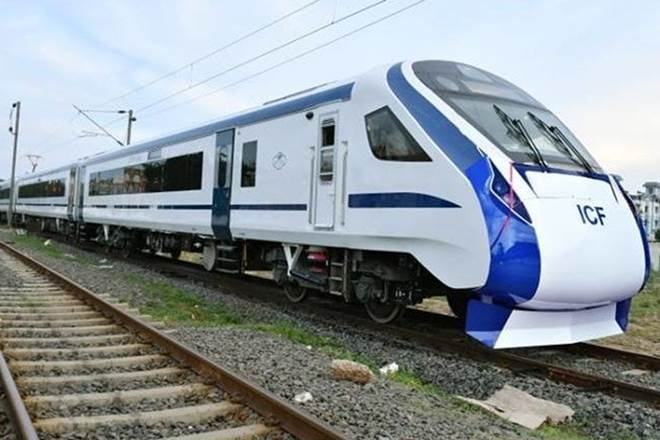
\includegraphics[height=0.50\textheight]{Figuras/Ch11/fig8}
\end{frame}


\begin{frame}{Correção da saída - Exemplo \#02}
	\begin{block}{}
		\begin{itemize}
			\item Um avião deve viajar a uma velocidade de \textbf{\SI{1500}{\kilo\meter\per\hour}} para completar seu itinerário a tempo e, após \textbf{turbulências}, sua velocidade se reduz para \textbf{\SI{1000}{\kilo\meter\per\hour}}.
			\item O controlador manda um sinal \textbf{proporcional} a essa diminuição, incrementando a velocidade para \textbf{\SI{1650}{\kilo\meter\per\hour}}.
			\item Após outra correção, sua velocidade se aproxima de \textbf{\SI{1400}{\kilo\meter\per\hour}}.
			\item Ainda longe do \textit{setpoint}, o controlador corrige sua saída \textbf{mais 5 vezes} até chegar em \textbf{\SI{1500}{\kilo\meter\per\hour}}.
		\end{itemize}
	\end{block}

	\centering
	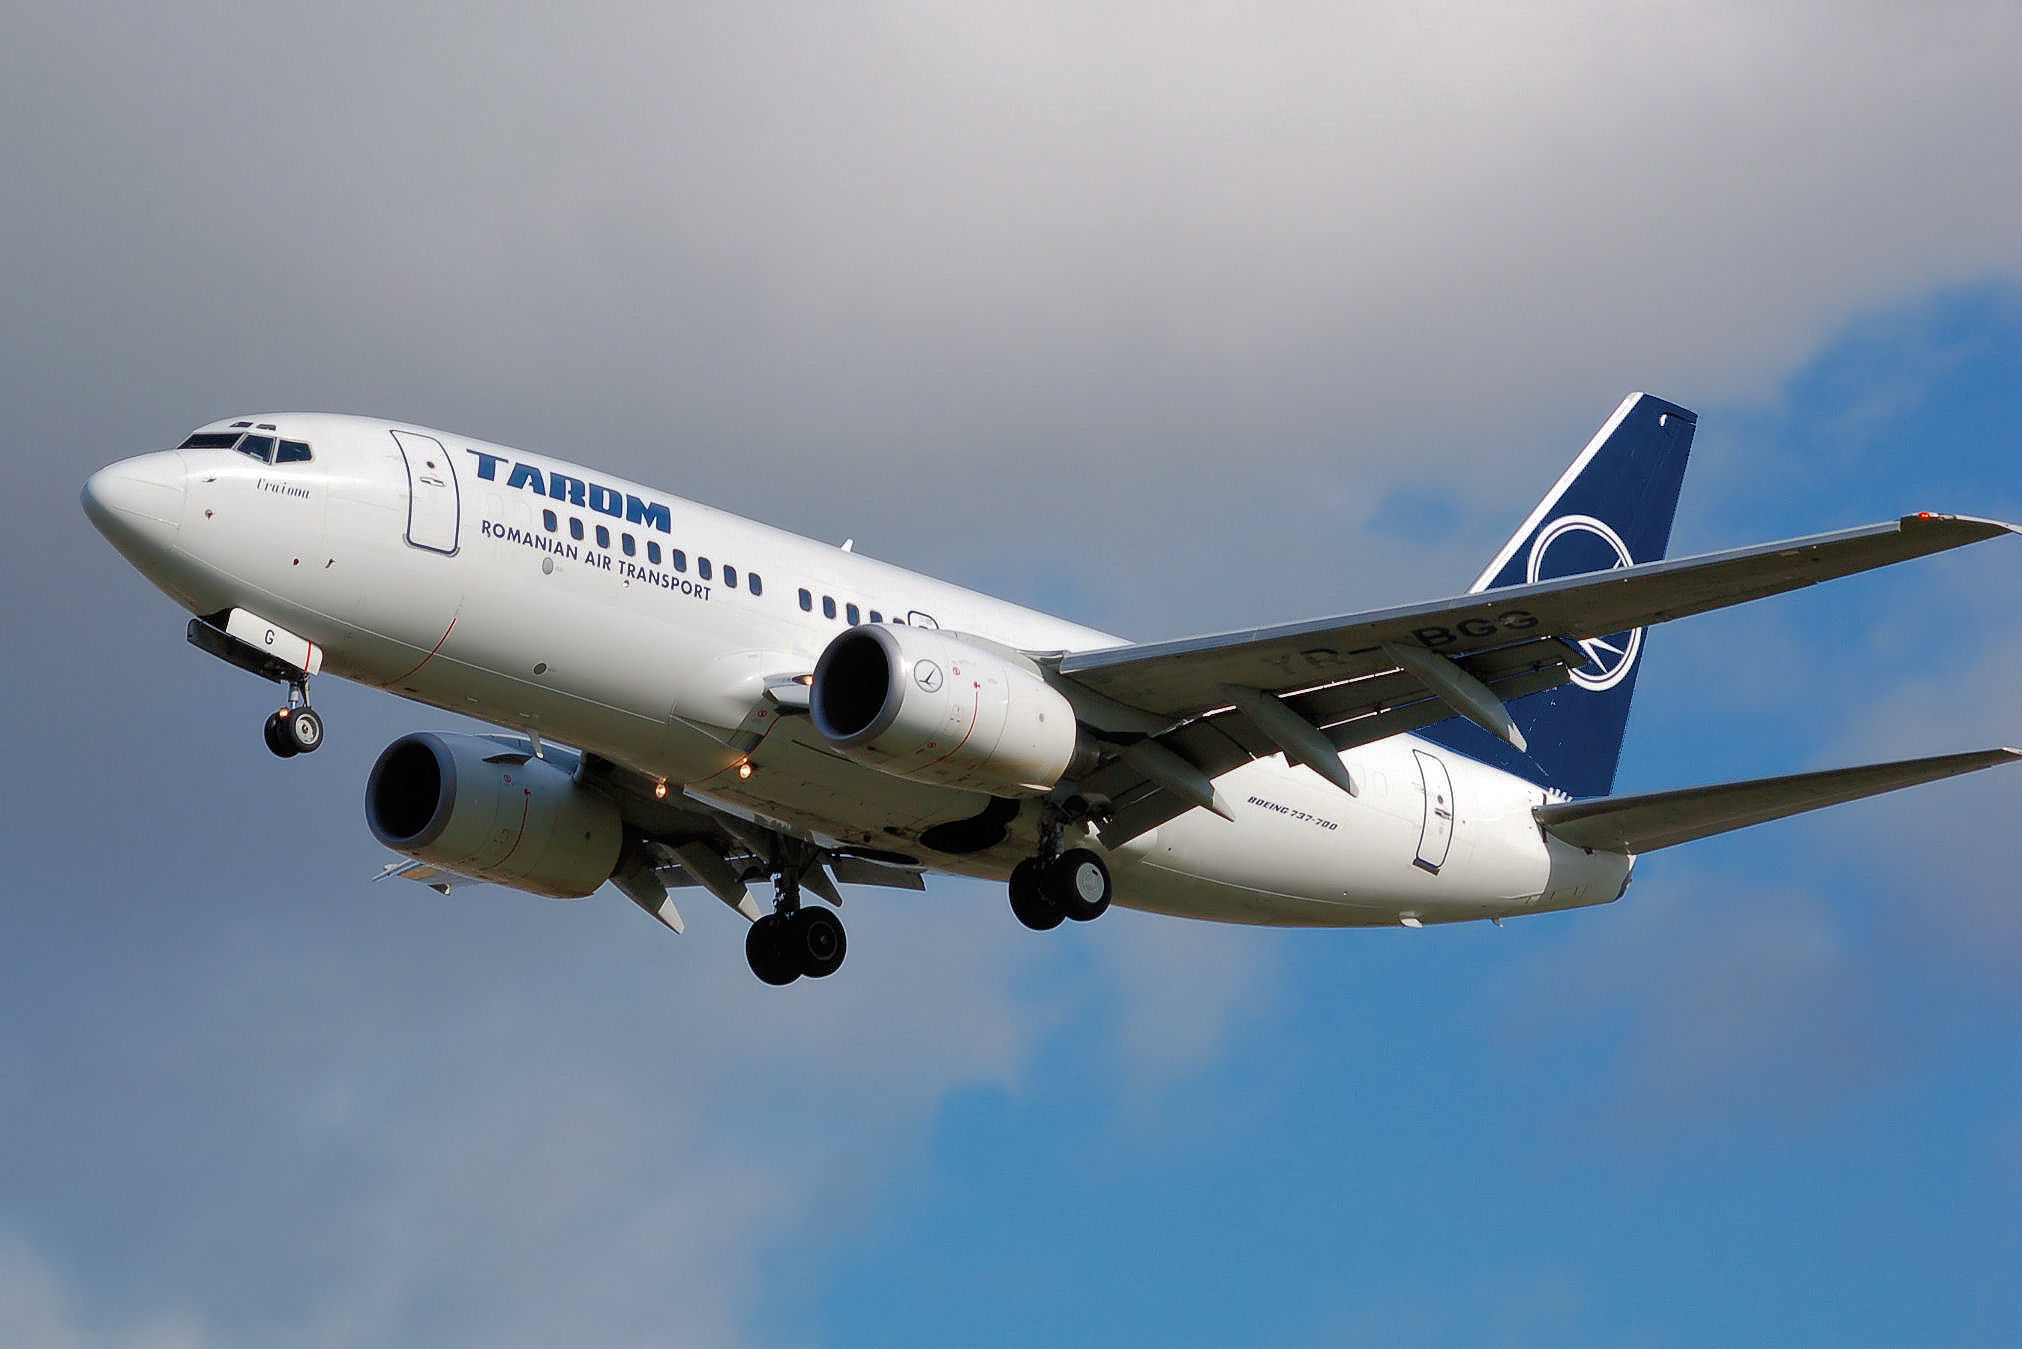
\includegraphics[height=0.4\textheight]{Figuras/Ch11/fig9}
\end{frame}


\begin{frame}{Correção da saída}
	\begin{block}{}
		Os dois exemplos apresentados usam valores múltiplos e, provavelmente, um método de controle similar, mas o segundo precisa realizar \textbf{bem mais} correções para chegar num \textbf{valor razoável}.
		
		\medskip
		
		Isso se deve à escala do problema, e podemos estudar alguns pontos importantes a partir destes dois casos:
		\begin{itemize}
			\item Regime \textbf{transitório} x regime \textbf{permanente}.
			\item Ações de controle.
		\end{itemize}
	\end{block}
\end{frame}


\begin{frame}{Correção da saída}
	\begin{block}{Regime transitório x regime permanente}
		\begin{itemize}
			\item É importante notar que a natureza do processo impacta \textbf{diretamente} sua \textbf{velocidade de resposta} a alterações \textbf{externas}.
			\item O nível de um reservatório grande (represa), por exemplo, pode levar \textbf{dias} para variar \textbf{significativamente}.
			\item Visto isso, é importante levar em conta o tempo necessário para a \textbf{variável controlada} se adequar às mudanças proporcionadas pelo controlador, que \textbf{nem sempre pode alterá-la diretamente}.
			\item Esse tempo de resposta é chamado \textbf{tempo morto}.
			\item Para corrigir variáveis que necessitam de \textbf{ação imediata} (velocidade de um trem) precisamos de \textbf{medidas drásticas}.
			\item A essas medidas denominamos \textbf{overshoot}, que seria uma resposta exagerada a fim de mudar o estado da variável \textbf{o mais rápido possível}.
		\end{itemize}
	\end{block}
\end{frame}


\begin{frame}{Correção da saída}
	\begin{block}{Regime transitório x regime permanente}
		\begin{itemize}
			\item Quanto \textbf{maior} o tempo morto e o overshoot, \textbf{mais difícil} se torna o controle de uma dada variável, visto que precisaremos de \textbf{mais tempo} para perceber alterações e \textbf{mais correções} no caminho para chegar ao \textit{setpoint}.
			\item Esse período de adaptações sem estabilidade se chama \textbf{regime transitório}, e é essencial que seja o \textbf{mais curto possível}.
			\item Quando \textbf{cessa} o regime transitório, começa o \textbf{regime permanente}, que é quando há certa \textbf{estabilidade}.
		\end{itemize}
	\end{block}
\end{frame}


\begin{frame}{Correção da saída}
	
	\centering
	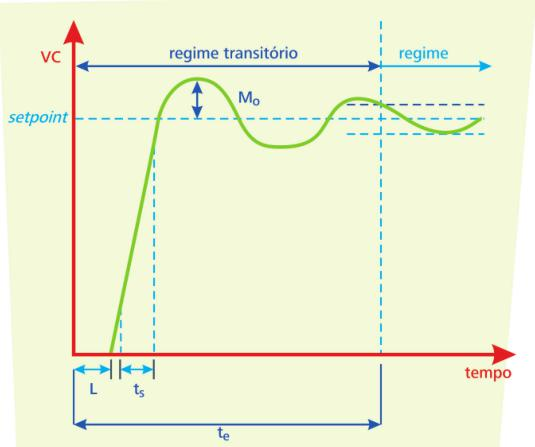
\includegraphics[width=0.7\linewidth]{Figuras/Ch11/fig10}
	
\end{frame}


\begin{frame}{Correção da saída}
	\begin{block}{Regime transitório x regime permanente}
		\begin{itemize}
			\item $ \bm{M_o} $ \textbf{-- Pico da resposta ou overshoot}
			
			É o \textbf{quanto} a variável controlada ultrapassa o \textit{setpoint} na primeira oscilação.
			\item $ \bm{t_e} $ \textbf{-- tempo de estabilização ou acomodação}
			
			Tempo que a variável controlada do processo demora para \textbf{alcançar 95\%} de seu valor em regime permanente (\textit{setpoint}).
			\item $ \bm{t_s} $ \textbf{-- tempo de subida}
			
			Tempo decorrido para que a variável controlada vá de \textbf{10\% até 90\% do \textit{setpoint}}.
			\item $ \bm{L} $ \textbf{-- Atraso ou tempo morto}
			
			Tempo que o processo leva para \textbf{começar a responder} a uma variação na variável manipulada.
		\end{itemize}
	\end{block}
\end{frame}


\frame{
	\frametitle{Exercícios}
	\begin{block}{}
		01. Monte o diagrama em blocos para os dois exemplos abordados anteriormente.
		
		\vspace{0.5cm}
		
		02. Esboce um gráfico de um processo onde $ SP=\SI{200}{\psip}, M_o=25\%,t_e=\SI{10}{\second},L=\SI{2}{\second} $ e $ t_s=\SI{2}{\second} $.
	\end{block}
}


\section*{Referências}
\frame{
	\frametitle{Referências e Exercícios Complementares}
	\begin{itemize}
		\item BAYER, Fernando Mariano; ARAÚJO, Olinto César Bassi de. Controle Automático de Processos, 3 ed. UFSM : Colégio Técnico Industrial de Santa Maria, 2011.
	\end{itemize}
	%\centering{\alert{Página 546 - \textbf{Capítulo 6}}} \\
	%\centering{\alert{Lista de exercícios 01}}
}